\documentclass{article}
\usepackage[T1]{fontenc}
\usepackage[polish]{babel}
\usepackage[utf8]{inputenc}
\usepackage{biblatex}
\usepackage{titling,lipsum}
\usepackage{indentfirst}
\usepackage{graphicx}
\usepackage{geometry}
\usepackage{float}

\addbibresource{bibliography.bib}

\title{Grafy i sieci - wykrywanie społeczności\\dokumentacja końcowa}
\date{\today}
\author{Ireneusz Stanicki, Mateusz Śliwakowski,\\Bartłomiej Truszkowski, Przemysław Woźniakowski}

\begin{document}
	\begin{titlingpage}
		\maketitle
	\end{titlingpage}
	\pagenumbering{arabic}

\tableofcontents
\newpage

%-----------------------------------------------------%
%Wstęp
%-----------------------------------------------------%
\section{Wstęp}
Problem wykrywania społeczności w sieciach okazał się być bardzo ciekawym, a jendocześnie przystępnym zagadnieniem. W ramach poniższego opracowania przedstawiamy opis czterech zaimplementowanych przez nas algorytmów wraz z modyfikacjami, informacje na temat zebranych przez nas danych oraz wyniki działania. Postaramy się przybliżyć jakie problemy napotkaliśmy podczas pracy, czy otrzymane rezultaty są zgodne z oczekiwaniami przedstawionymi w dokumentacji wstępnej oraz jakie wnioski można wyciągnąć po przeprowadzonych eksperymentach.

%-----------------------------------------------------%
%Algorytmy
%-----------------------------------------------------%
\section{Algorytmy}

%-----------------------------------------------------%
%Girvan Newman
%-----------------------------------------------------%
\subsection{Algorytm Girvan-Newmana}
\subsubsection{Implementacja}

W przypadku tego algorytmu praca została rozpoczęta od podstaw, a więc tradycyjnej wersji algorytmu Girvan-Newman dla społeczności rozłącznych. Jak się okazało biblioteka igraph, z której korzystaliśmy, udostępnia wbudowaną funkcję do wyliczania parametru edge betweenness. Dzięki skorzystaniu z tej metody implementacja algorytmu sprowadziła się do krótkiej funkcji, która wyznacza ww. parametr, a następnie usuwa krawędź, dla której jest on największy. Algorytm ten nie podlegał dalszej analizie - wykorzystano go tylko do sprawdzenia poprawności danych, na których pracowaliśmy, a także określenia struktury wyniku użytej w całym algorytmu.\\
Aby uzyskać wynik w postaci społeczności nachodzących użyty został algorytm CONGA, do którego zastosowano własne modyfikacje. Także w tym wypadku pomocna okazała się biblioteka igraph, w której zaimplementowana jest funkcja do wyznaczania parametru vertex betweenness. Dzięki temu w każdym kroku uzyskano zbiory dwóch kluczowych parametrów dla przebiegu całego algorytmu.\\
Warto przybliżyć również strukturę wyniku, który był zwracany przez zmodyfikowany algorytm. Funkcja zwracała tablicę wartości modularnośći dla każdego z kroku algorytmu. Ponadto uzupełniana była także tablica tablic results, która zawierała wyjściowy dendrogram. Po wykonaniu kroku algorytmu do results doklejana była kolejna tablica, zawierającą krawędzie usunięte w danym kroku. W przypadku konstrukcji tej tablicy przyjęto następującą zasadę: gdy dochodziło do kopiowania wierzchołka pierwszą krawędź stanowiła pętle dla wierzchołka kopiowanego.\\
Chcąc odtworzyć rozwiązanie dla danego kroku z dendrogramu wyjściowego, konieczne było użycie tablicy Overlap, która również była uzupełniana w trakcie działania programu. Dla oryginalnych wierzchołków wartość w tej tablicy wynosiła -1, dla dodawanych wskazywała na numer wierzchołka, z którego został on skopiowany.\\
Wynik działania funkcji musiał jeszcze zostać zmodyfikowany w celu uzyskania najlepszego wyniku dla badanego grafu. Dzięki temu opierając się na współczynniku modularności określana była wartość docelowa dla danego grafu (więcej na temat w kolejnej sekcji). Następnie z wyjściowego dendrogramu graf był odtwarzany do kroku, któremu odpowiadał użyty parametr modularności. Kolejną część stanowiła modyfikacja takiego grafu do wizulizacji - konieczne było tutaj połączenie wszystkich kopii wierzchołków, przy zachowaniu odpowiednich numerów społeczności.

\subsubsection{Podjęte decyzje}
Pierwszą decyzję, jaką należało podjąć przy implementacji algorytmu, był wybór sposobu obliczania modularności. Miara ta jest jasno określona przez autorów oryginalnego algorytmu Girvan-Newman, lecz przy modyfikacjach dla społeczności nachodzących nie dysponujemy tego typu wzorem. Wobec tego jako miara modularności został wybrany tutaj wskaźnik użyty w przypadku algorytmu OCDLCE, który został odpowiednio dostosowany do algorytmu CONGA. Miara ta skupiona jest na jednej społeczności lokalnej, natomiast w opisywanym przypadku należało ją określić dla całego grafu. Wobec czego była ona wyliczana dla każdej uzyskanej społeczności, a następnie aby określić modularność dla całego grafu, posłożono się średnią arytmetyczną z uzyskanych wartości. \\
Kolejny ważny wybór dotyczący modularności opierał się na wyborze tej wartości, dla której uzyskany wynik jest najlepszy. Założenie początkowe miary z OCDLCE opierało się na tym, iż rezultat jest najlepszy wtedy, gdy największa jest wartość tego parametru. W wypadku algorytmu CONGA również można skorzystać z takowego założenia, jednak nie można zapominać o plusach tego algorytmu, a więc łatwego odzyskiwania społeczności wynikowych w zależności od preferencji co do ich rozmiaru/kształtu. Aby to umożliwić, zdecydowano się na wybór maksimów lokalnych dla całej tablicy wartości modularności. Następnie z wybranych wartości dokonywano wyboru wartości wynikowej na podstawie określonego na wejściu kwantylu. Tą wartością można już było manipulować - im mniejsza jej wartość tym bardziej wynikowa społeczność była rozrzedzona. I analogicznie - chcąc otrzymać podział na większe grupy należało zwiększyć tę wartość.\\
Manipulację liczbą społeczności, jaką chcemy otrzymać, można było także uskutecznić przy pomocy preprocessingu. Polegał on na przejściu całego grafu przez algorytm, z tą różnicą, że jedyną zwracaną wartością była tablica różnic pomiędzy wartościami edge i vertex betweenness. Bazując na wartościach z każdego kroku można było określić, jaki stopień rozdrobnienia społeczności chcemy uzyskać. W ten sposób do głównego wykonania programu można było przesłać parametr gap, który określał handicap, jaki dajemy usuwaniu krawędzi nad kopiowaniem wierzchołka. Im większą wartość dla tego parametru wybraliśmy z wyniku preprocessingu, tym społeczności wynikowe były liczniejsze (co jednak zależało także od wyboru końcowego, wspomnianego w poprzednim akapicie).\\
Przechodząc do esencji algorytmu należy wspomnieć o dokonanych własnych modyfikacjach. Początkowo założono, iż dla tego algorytmu modyfikacje będziemy stosować w procesie kopiowania wierzchołka. Zgodnie z tymi założeniami zaimplementowane zostały dwa rozwiązania. Pierwsze z nich stosuje podział wierzchołka wyłącznie na podstawie daty zawarcia znajomości. W ten sposób wyliczamy średnią z dat zawarcia znajomości dla każdej z incydentnych krawędzi danego wierzchołka, a następnie te z wartościami poniżej średniej 'przepinamy' do kopii wierzchołka, resztę pozostawiając z oryginałem.\\
Podobnie postępujemy w przypadku modyfikacji używającej liczby wspólnych znajomych. W tym wypadku zmieniony został jednak sposób wyliczania wartości, która stanowi odniesienie porównania przy dzieleniu. Dla danego wierzchołka wyliczana jest tutaj średnia ważona, gdzie wagę stanowi liczba wspólnych znajomych. O ile pierwszy sposób wyliczania powinien premiować prosty podział chronologiczny, tak w tym wypadku większy nacisk powinien zostać położony na bardziej zżyte ze sobą społeczności (osoby, które niekoniecznie poznały się w danym czasie, ale dłużej znajdowały się wspólnie w danej grupie).\\
Usuwanie krawędzi w trakcie działania algorytmu dokonywano zbiorowo - wszystkie krawędzie, dla których wartość parametru edge betweenness była największa, były usuwane w jednym kroku algorytmu.\\

%-----------------------------------------------------%
%LPA
%-----------------------------------------------------%
\subsection{Label Propagation Algorithm}
\subsubsection{Implementacja}

Wersja podstawowa algorytmu Label Propagation była już zaimplementowana w bibliotece igraph. Pozostało jedynie dostosowanie jej wyniku tak, aby dało się go zwizualizować za pomocą naszej warstwy prezentacji. Jako że dalsze modyfikacje opierały się na tej wersji, konieczne okazało się również zaimplementowanie jej w naszym projekcie od podstaw.\\

Posiadając już podstawową wersję algorytmu pozostało zmodyfikować ją tak, aby była ona w stanie wykrywać społeczności nachodzące. Zgodnie z dokumentacją początkową wprowadzono parametr, określający maksymalną liczbę społeczności, do której może przynależeć wierzchołek i zmodyfikowano krok algorytmu tak, aby był w stanie przypisać rozpatrzanemu wierzchołkowi więcej niż jedną społeczność.\\

W ramach tego opracowania nie udało się wprowadzić modyfikacji z parametrem znormalizowanym. Okazało się jednak, że kroki z innych algorytmów można połączyć z algorytmem LPA. Tak więc wykorzystano krok pierwszy algorytmu OCDLCE do inicjalizacji początkowych społeczności algorytmu LPA. Korzystając z faktu, że algorytm LPA jest niedeterministyczny, można było również użyć ostatniego kroku algorytmu Louvein do połączenia kilku rozwiązań rozłącznych w takie, gdzie społeczności są nachodzące.\\

Modyfikacje związane z dodatkowymi własnościami grafu zostały zrealizowane zgodnie z założeniami. Dla dat zawarcia znajomości algorytm opiera się na odchyleniu standardowym - wybiera społeczność, gdzie jest ono najmniejsze. Przy liczbie wspólnych znajomych, czy innym parametrze ilościowym (np. liczba commitów w pracy nad wspólnym repozytorium), wybierana jest grupa, gdzie suma dla tego parametru jest maksymalna.

\subsubsection{Podjęte decyzje}

W podstawowej wersji algorytmu dużym problemem była oscylacja w grafach bliskich dwudzielnym. Aby zapobiec temu problemowi wprowadzono zabezpieczenie - jeżeli obecna społeczność wierzchołka znajduje się w zbiorze społeczności, między którymi rozpatrujemy remis, to wybieramy ją jako zwycięską.\\

Kolejnym problemem, okazało się (zgodnie z oczekiwaniami) formowanie społeczności gigantycznych. Szczególnie brak zabezpieczeń tego typu był widoczny w implementacji wbudowanej w bibliotekę igraph, gdzie nawet dla niezbyt gęstych grafów algorytm często umieszczał wszystkie wierzchołki w jednej społeczności. Problem ten nie został rozwiązany wprost w naszej implementacji, ponieważ umożliwiono określanie maksymalnej liczby iteracji, co skutecznie pozwala na ograniczenie maksymalnej wielkości społeczności.\\

Zaimplementowano prostą wersję algorytmu używającej technologi CUDA. Implementacja ta powstała w celach porównawczych pod kątem czasu wykonania, zatem nie były w niej wprowadzane żadne modyfikacje. Ze względu na architekturę konieczne było również ograniczenie liczby przetwarzanych społeczności dla danego wierzchołka. Aby ograniczyć użycie pamięci lokalnej wątków zdecydowano się na rozpatrywanie maksymalnie 64 etykiet dla pojedynczego wierzchołka. W implementacji tej skupiono się wyłącznie na fazie obliczeń. Przekształcanie reprezentacji grafu zaimplementowano naiwnie, jako że nie jest ono istotna w rozważaniach.

%-----------------------------------------------------%
%OCDLCE
%-----------------------------------------------------%
\subsection{Overlapping Community Detection by Local Community Expansion}
\subsubsection{Implementacja}
\subsubsection{Podjęte decyzje}

%-----------------------------------------------------%
%Louvain
%-----------------------------------------------------%
\subsection{Algorytm Louvain}

\subsubsection{Implementacja}
Algorytm Louvain został zaimplementowany od podstaw. Pierwszym krokiem było dodanie wszystkich funkcji pomocniczych, koniecznych do obliczenia wartości takich jak liczba połączeń do społeczności (nie wliczając pętli) czyli $\Sigma_{tot}$, liczba połączeń wewnątrz społeczności czyli $\Sigma_{in}$, czy liczba połączeń do wierzchołka k rozpatrywanej społeczności $k_{in}$. Funkcje te wywoływane są tylko w koniecznych sytuacjach. W miarę możliwości odpowiednie parametry są uaktualniane, zamiast ciągłego ich przeliczania.\\ \\
Podstawą algorytmu jest funkcja $louvain\_ iteration$, która odpowiada pojedynczej iteracji algorytmu. Jej zadaniem jest uaktualnianie tablicy przynależności, która mówi w jakiej społeczności aktualnie znajduje się wierzchołek.\\ Na początku wyznaczana jest w niej suma wag krawędzi w grafie i tworzona jest kopia tablicy przynależności, a następnie za pomocą pętli iterujemy po wszystkich wierzchołkach. Kolejność rozpatrywania wierzchołków zależy od tablicy $permut$, która jest losową permutacją liczb od $1$ do $n$ ($n$-liczba wierzchołków). \\Dla każdego wierzchołka rozpatrywane są społeczności do których należą jego sąsiedzi (każda społeczność jest brana pod uwagę tylko raz). Wierzchołek jest usuwany ze swojej społeczności i umieszczany w społeczności sąsiada, a następnie obliczany jest przyrost modularności. Jeżeli przyrost dla społeczności jest większy od aktualnego maksymalnego przyrostu ($max\_ mod\_ change$) to staje się on nowym maksymalnym przyrostem, a społeczność ta jest zapamiętywana. Następnie wierzchołek wraca do swojej społeczności i proces jest powtarzany dla każdego sąsiada. \\
Warto tu przypomnieć wzór na zmianę modularności: $$\Delta Q = [\frac{\Sigma_{in} +2k_{i,in}}{2m} - (\frac{\Sigma_{tot} + k_i}{2m})^2] - [\frac{\Sigma_{in}}{2m} - (\frac{\Sigma_{tot}}{2m})^2 - (\frac{k_i}{2m})^2]$$ gdzie $k_i$ to stopień wierzchołka $i$, $k_{in}$ to suma wag krawędzi między wierzchołkiem $i$ i wierzchołkami ze społeczności, do której trafia $i$, $\Sigma_{in}$ to suma wag krawędzi wewnątrz tej społeczności, a $\Sigma_{tot}$ to suma wag krawędzi wewnątrz społeczności z której usuwamy wierzchołek $i$.\\Jest to jednak rozpisany wzór i w implementacji wykorzystana jest jego skrócona wersja: $$\Delta Q = [\frac{k_{i,in}}{m} - \frac{\Sigma_{tot}*k_i}{2m^2}]$$ \\
\\
Po przeiterowaniu wszystkich sąsiadów wierzchołka, sprawdzane jest czy znaleziono społeczność zwiększającą modularność, która nie jest oryginalną społecznością wierzchołka. Jeżeli tak jest, to odnotowywana jest zmiana, oraz uaktualniane są odpowiednie wartości i tablica przynależności (zarówno dla danego wierzchołka, jak i dla wszystkich, które zostały z nim scalone).
\\
Po przejściu wszystkich wierzchołków, tablica przynależności jest podmieniana i zwracana jest wartość logiczna, mówiąca czy nastąpiła zmiana.  
\\
Równie ważna funkcją w algorytmie jest funkcja scalająca wierzchołki znajdujące się w jednej społeczności - $merge\_ communities$. Tworzy ona nowy graf, w którym każdej społeczności odpowiada wierzchołek umieszczony w tej społeczności. Suma wag krawędzi między wierzchołkami wewnątrz społeczności staje się pętlą w nowym grafie, a suma krawędzi między społecznościami wagą krawędzi pomiędzy odpowiadającymi im wierzchołkami.
\\ \\
Cały algorytm wykonywany jest w funkcji $louvain\_ algorithm$. Wyznaczana jest w niej wartość $\Sigma_{tot}$ dla każdej społeczności, tworzona jest kopia grafu oraz każdy wierzchołek umieszczany jest w swojej społeczności. Następnie w pętli wykonywana jest funkcja $louvain\_ iteration$, tak długo jak powoduje ona jakieś zmiany społeczności. Po każdej iteracji społeczności są scalane. Wynikiem algorytmu jest tablica przynależności. Algorytm nie modyfikuje oryginalnego grafu.

\subsubsection{Implementacja dla nachodzących społeczności}
Algorytm dla społeczności nachodzących wykorzystuje algorytm dla społeczności rozłącznych. Został przede wszystkim zaimplementowany do współpracy z algorytmem Louvaina, ale może działać też z innym nie deterministycznymi algorytmami. Muszą one jednak zwracać tablicę przynależności. \\
Celem algorytmu jest skonstruowanie macierzy przynależności. Jest to macierz $n \times k$, gdzie $n$ to ilość wierzchołków, a $k$ to ilość społeczności. Element $[i][j]$ oznacza jak bardzo wierzchołek i należy do społeczności j.
\\ Algorytm rozpoczyna się od pojedynczego przebiegu algorytmu dla społeczności rozłącznych. Jego wynikowa tablica jest tłumaczona tak aby numery społeczności były liczbami od $0$ do $k-1$ ($k$ -ilość społeczności w wyznaczonym podziale). Będzie podstawą do wygenerowania macierzy przynależności. Jest ona od razu aktualizowana. Do elementu $[i][j]$ dodajemy ilość połączeń wierzchołka $i$ z wierzchołkami ze społeczności $j$.\\
Następnie wywołujemy algorytm dla społeczności rozłącznych określoną ilość razy. Po każdym przebiegu wynikowa tablica jest tłumaczona, tak by społeczności odpowiadające tym w tablicy z oryginalnego przebiegu miały ten sam numer. W tym celu dla każdej społeczności znajdowana jest taka, w której ilość pokrywających się wierzchołków jest największa. Następnie macierz przynależności jest aktualizowana, analogicznie jak po początkowym przebiegu.\\ 
Po wykonaniu założonych przebiegów, macierz przynależności jest normalizowana (tak by suma współczynników dla każdego wierzchołka wynosiła 1). Następnie każdemu wierzchołkowi przydzielane są społeczności, dla których współczynnik przynależności przekroczył wartość progową (obliczaną na podstawie parametru funkcji). Współczynniki dla społeczności, które nie przekroczyły wartości progowej są zerowane, a macierz znów jest normalizowana. Jeżeli wierzchołek dla wszystkich społeczności ma współczynnik 0 (tzn. jest wyizolowany), to jest on przydzielany do swojej społeczności. Jeżeli dla wierzchołka, żaden ze współczynników nie przekroczy wartości progowej, to umieszczany jest on w społeczności z największym współczynnikiem. Jest to rozwiązanie na swój sposób prowizoryczne. Takie wierzchołki mogą być bowiem czasami łącznikami pomiędzy społecznościami i w takich sytuacjach wypadałoby umieścić je we wszystkich społecznościach. Jest to jednak problem, który nie został poruszony w tej implementacji i może być obiektem usprawnień w przyszłości.
\subsubsection{Podjęte decyzje}
Metoda dla społeczności nachodzących opisana w artykule "A Fast Algorithm for Overlapping Community Detection" \cite{pw-paper3}, zakładała obecność jeszcze jednego kroku, którego celem miała być ogólna poprawa jakości wyniku. Metoda ta opierała się jednak na modularności Nicosii \cite{pw-paper2}, której obliczenie jest na tyle kosztowne, że zwiększa złożoność algorytmu do $n^3$. Z racji, że zdecydowanie pogorszyło by to czas obliczeń i negatywnie wpłynęło na możliwość wielokrotnego testowania (zwłaszcza dla grafów o kilku tysiącach wierzchołków), a także biorąc pod uwagę fakt, że wyniki bez tego kroku były zadowalające, postanowiliśmy z niego zrezygnować.\\\ Dodatkową modyfikacją jest możliwość przekazywania  opcjonalnego parametru do wywołania funkcji $louvain\_ algorithm$. Parametr ten wpływa na to jak bardzo element $\frac{\Sigma_{tot}*k_i}{2m^2}$ wpływa na zmianę modularności. Dla wartości mniejszych promuje on powstawanie niewielu, rozległych społeczności, a dla większych - powstawanie wielu drobniejszych społeczności. Najlepsze wartości modularności uzyskiwane są co prawda dla wartości 1, ale parametr pozwala na dostosowywanie wyniku do naszych oczekiwań, przy nieznacznych stratach na jakości.

%-----------------------------------------------------%
%Dane testowe
%-----------------------------------------------------%
\section{Dane testowe}
Rozpoczynając pracę, zakładaliśmy, że opisane algorytmy będziemy badać na zbiorach danych udostępnianych przez firmę Facebook. Portal ten chyba najbardziej kojarzy się z ogromnym źródłem danych dotyczących społeczności. Niestety modyfikacje, które chcieliśmy zastosować, nie mogły zostać zrealizowane na datasetach ściągniętych z tego portalu. Żaden z szeroko dostępnych zbiorów nie zawierał informacji na temat liczby wspólnych znajomych, a także daty zawarcia znajomości. O ile zdobycie tej pierwszej wiadomośći jest bardzo proste przy użyciu nawet najbardziej naiwnego algorytmu brute force, tak uzyskanie dat można było przeprowadzić tylko w sposób losowy, co mogło by tylko zaburzyć osiągane wyniki. Wobec tego swe spojrzenie skierowaliśmy w stronę zbiorów, które na pierwszy rzut oka nie kojarzą się ze społecznościami tak dobrze jak Facebook.
%-----------------------------------------------------%
%NBA
%-----------------------------------------------------%
\subsection{NBA}
'I love this game' - to slogan reklamowy towarzyszący najlepszej lidze koszykarskiej, który odnosi się także do jednego z autorów tej pracy. Wybór tego zbioru danych motywowany był prywatnymi zainteresowaniami autorów, które wiążą się także z ogólną wiedzą na temat samej ligi. Dzięki temu zyskaliśmy możliwość oceny osiąganych rezultatów 'ludzkim okiem', przez co można było je poprawiać i oceniać dzięki swego rodzaju eksperckiej wiedzy na temat NBA.\\
Swoją rolę odegrała tu także ogólna dostępność danych. Ich źródło stanowił portal basketball-reference.com, który stanowi internetową, koszykarską encyklopedię. Korzystając ze scrapera napisanego w języku JavaScript można było zautomatyzować proces wyszukiwania danych. Pomógł tutaj alfabetyczny spis koszykarzy - w ten sposób zdobyliśmy informację na temat każdego z nich, a także w łatwy sposób uzyskaliśmy liczbę wszystkich sezonów i klubów, w jakich w swojej karierze występował dany zawodnik. Następnie dane te zostały obrobione z wykorzystaniem SQL, w celu uzyskania relacji między zawodnikami, a także daty zawarcia znajomości. Liczba wspólnych znajomych została określona przy pomocy prostego algorytmu napisanego w języku C\#.\\
Graf, który uzyskaliśmy, składa się z 4800 wierzchołków. Każdy wierzchołek można przypisać zawodnikowi, który postawił swą stopę na parkietach NBA w ciągu ponad 70 lat istnienia ligi. Dwaj zawodnicy są ze sobą w relacji, jeśli kiedykolwiek zagrali ze sobą w jednym klubie. Data zawarcia znajomości to w tym wypadku data pierwszego meczu, w którym obaj zawodnicy mieli okazję ze sobą zagrać. Tworząc relacje w ten sposób uzyskaliśmy ponad 146 tysięcy krawędzi.

%-----------------------------------------------------%
%Filmweb
%-----------------------------------------------------%
\subsection{Filmweb}
Poszukując parametru daty zawarcia znajomości zwróciliśmy się także ku innej części branży rozrywkowej. Źrodło danych w tym wypadku stanowił portal filmweb.pl, który dysponuje ogromną bazą danych na temat aktorów i filmów. Skala tych danych jest tak duża, iż musieliśmy ograniczyć nasze prace tylko do polskich aktorów. W ten sposób uzyskaliśmy graf z 10 000 wierzchołków i 190031 krawędziami.\\
Sposób uzyskania danych był analogiczny do tego prezentowanego w przypadku grafu NBA. Skonstruowany w języku JavaScript scraper został wykorzystany do przejrzenia listy wszystkich polskich aktorów, by następnie dla każdego z nich znaleźć listę kolegów z branży, z którymi najczęśniej występował w jednym filmie. Ten zbiór uczyniliśmy znajomymi badanego aktora. Datę zawarcia znajomości w tym wypadku stanowiła data premiery pierwszego filmu/serialu, w którym dana dwójka ze sobą wystąpiła. Dodatkowo na prośbę prowadzącego zbiór danych uzupełniony został o liczbę filmów, w których dana dwójka wspólnie występowała. Informacja ta okazała się również przydatna w modyfikacji jednego z algorytmów.\\
Podsumowując, wierzchołki uzyskanego grafu stanowią polscy aktorzy, pobrani z ogólnodostępnej bazy filmweb. Dwaj aktorzy są ze sobą w relacji, jeśli jeden z nich znajduje się w zakładce 'najczęściej występował z ...' u drugiego. Motywację wyboru tego grafu jako testowego stanowiło ogólne zainteresowanie branżą filmową autorów pracy, a także ogólna dostępność danych. Sama etykietyzacja wierzchołków pozwoliła nam łatwiej oceniać poprawność działania algorytmów - zwłaszcza w początkowej fazie implementacji z wykorzystaniem tylko małych zbiorów danych.

%-----------------------------------------------------%
%Github
%-----------------------------------------------------%
\subsection{GitHub}

%-----------------------------------------------------%
%Wyniki
%-----------------------------------------------------%
\section{Wyniki}

%-----------------------------------------------------%
%Girvan Newman
%-----------------------------------------------------%
\subsection{Algorytm Girvan-Newmana}
\subsubsection{Analiza czasowa}
Założenie polegające na tym, iż w każdym kroku liczone są najkrótsze ścieżki pomiędzy każdą parą wierzchołków okazało się kluczowe, jeśli patrzymy pod kątem czasu wykonania. Chcąc szybko osiągnąć wynik wybór algorytmu Girvan-Newman nie jest wyborem najlepszym już dla społeczności rozłącznych. Rozszerzając algorytm na społeczności nachodzące (przy pomocy algorytmu CONGA z własnymi modyfikacjami) jeszcze bardziej utrudniamy pracę algorytmowi, tworząc kopie wierzchołków i rozszerzając przez to zbiór par, dla których liczone są najkrótsze ścieżki.
\subsubsection{Analiza jakościowa}
Po wykonaniu analizy algorytmu, a przed przystąpieniem do implementacji, fakt jego wolnego działania nie został przez nikogo przyjęty ze zdziwieniem. Cechą, którą miał obronić się ten algorytm, była jakość rozwiązania. Rzeczywiście na tym polu można zauważyć, że algorytm zachowuje się o wiele lepiej z perspektywy użytkownika. Po wykonaniu pełnego przebiegu dla danego grafu i otrzymania wynikowego dendrogramu manipulacja wynikiem, którego poszukujemy, zależy już tylko od indywidualnych preferencji użytkownika.\\
Usystematyzować te preferencje pozwoliły metody wykorzystane w implementacji. Pierwszą z nich było określenie, którego z maksimów lokalnych poszukujemy. Na podstawie ich zbioru umożliwiony został wybór, który kwantyl wśród wyników, jest tym nas interesującym. Jeżeli otrzymany wynik nie był jednak zadowalający (np. ze względu na zbyt duży bądź zbyt mały rozmiar społeczności wynikowych), można było zmienić wartość kwantylu i wedle preferencji uzyskać podział na większe bądź mniejsze grupy.\\
Aby zaprezentować wyżej opisane własności najlepiej będzie posłużyć się przykładem. W tym celu skorzystam z grafu uczestników NBA All-Star Games w 4 ostatnich sezonach.

\begin{figure}[H]
\centering
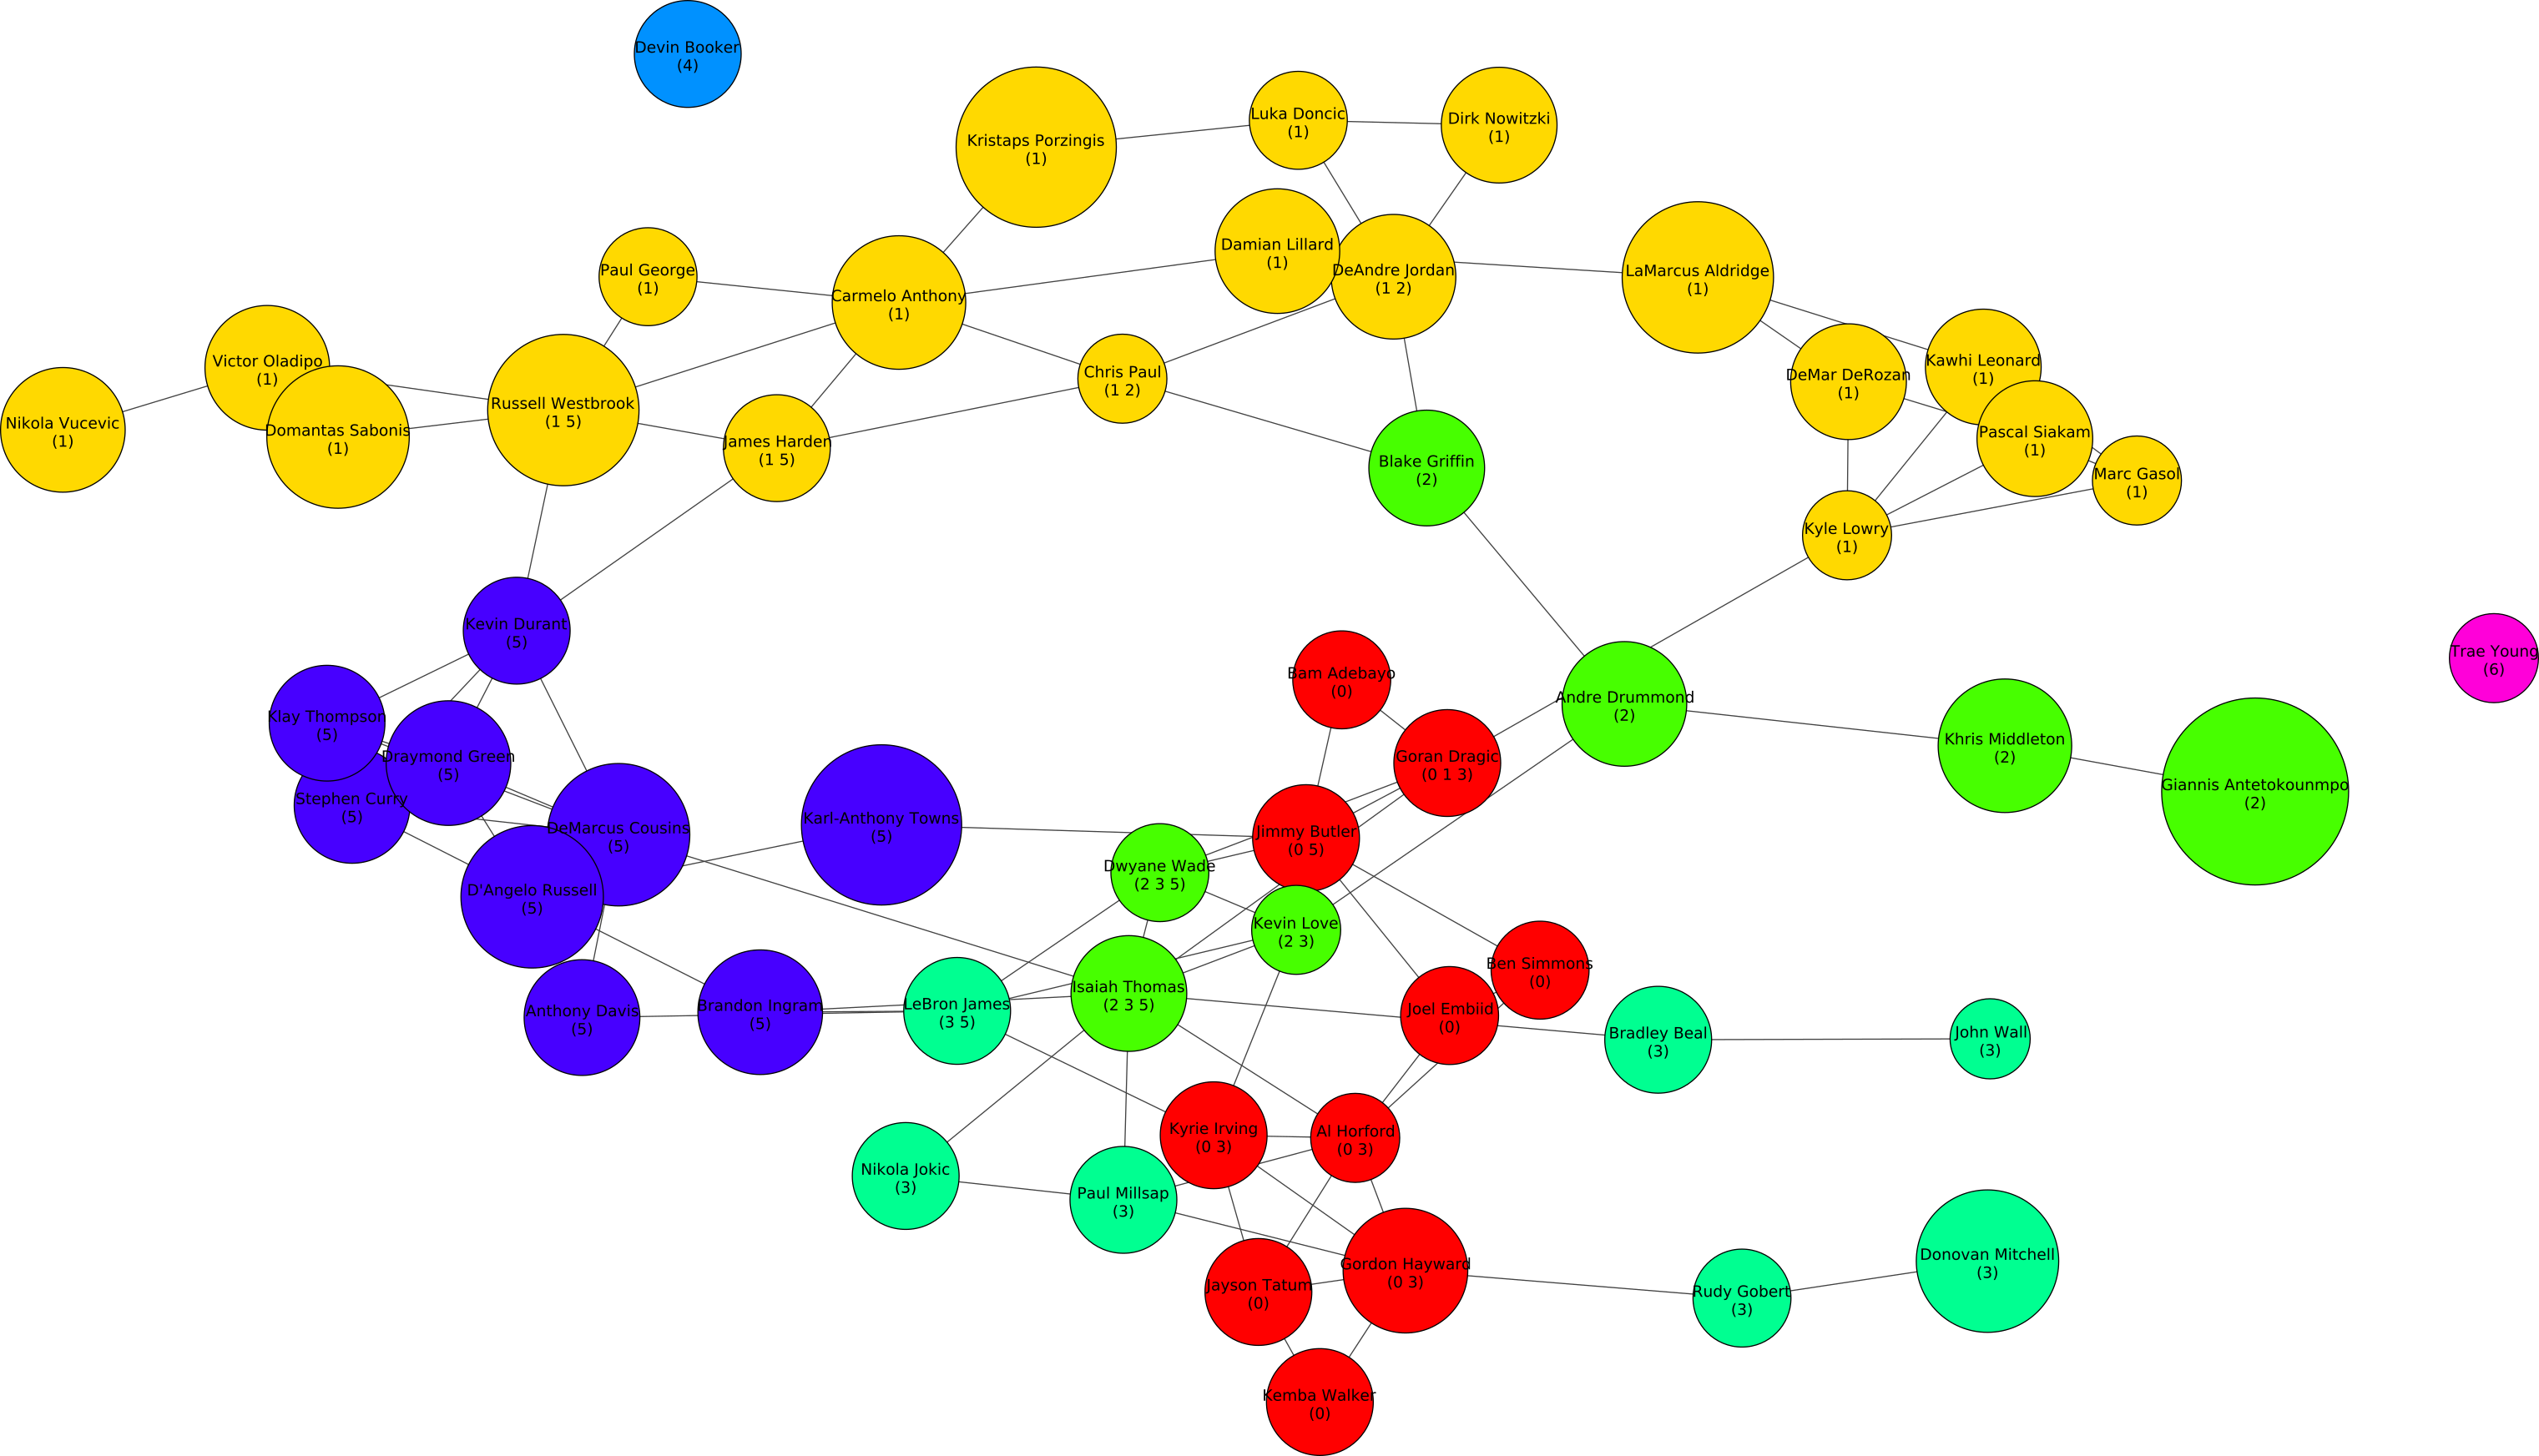
\includegraphics[width=\textwidth]{images/is-sample-1.png}
\caption{Największa modularność}
\end{figure}

\begin{figure}[H]
\centering
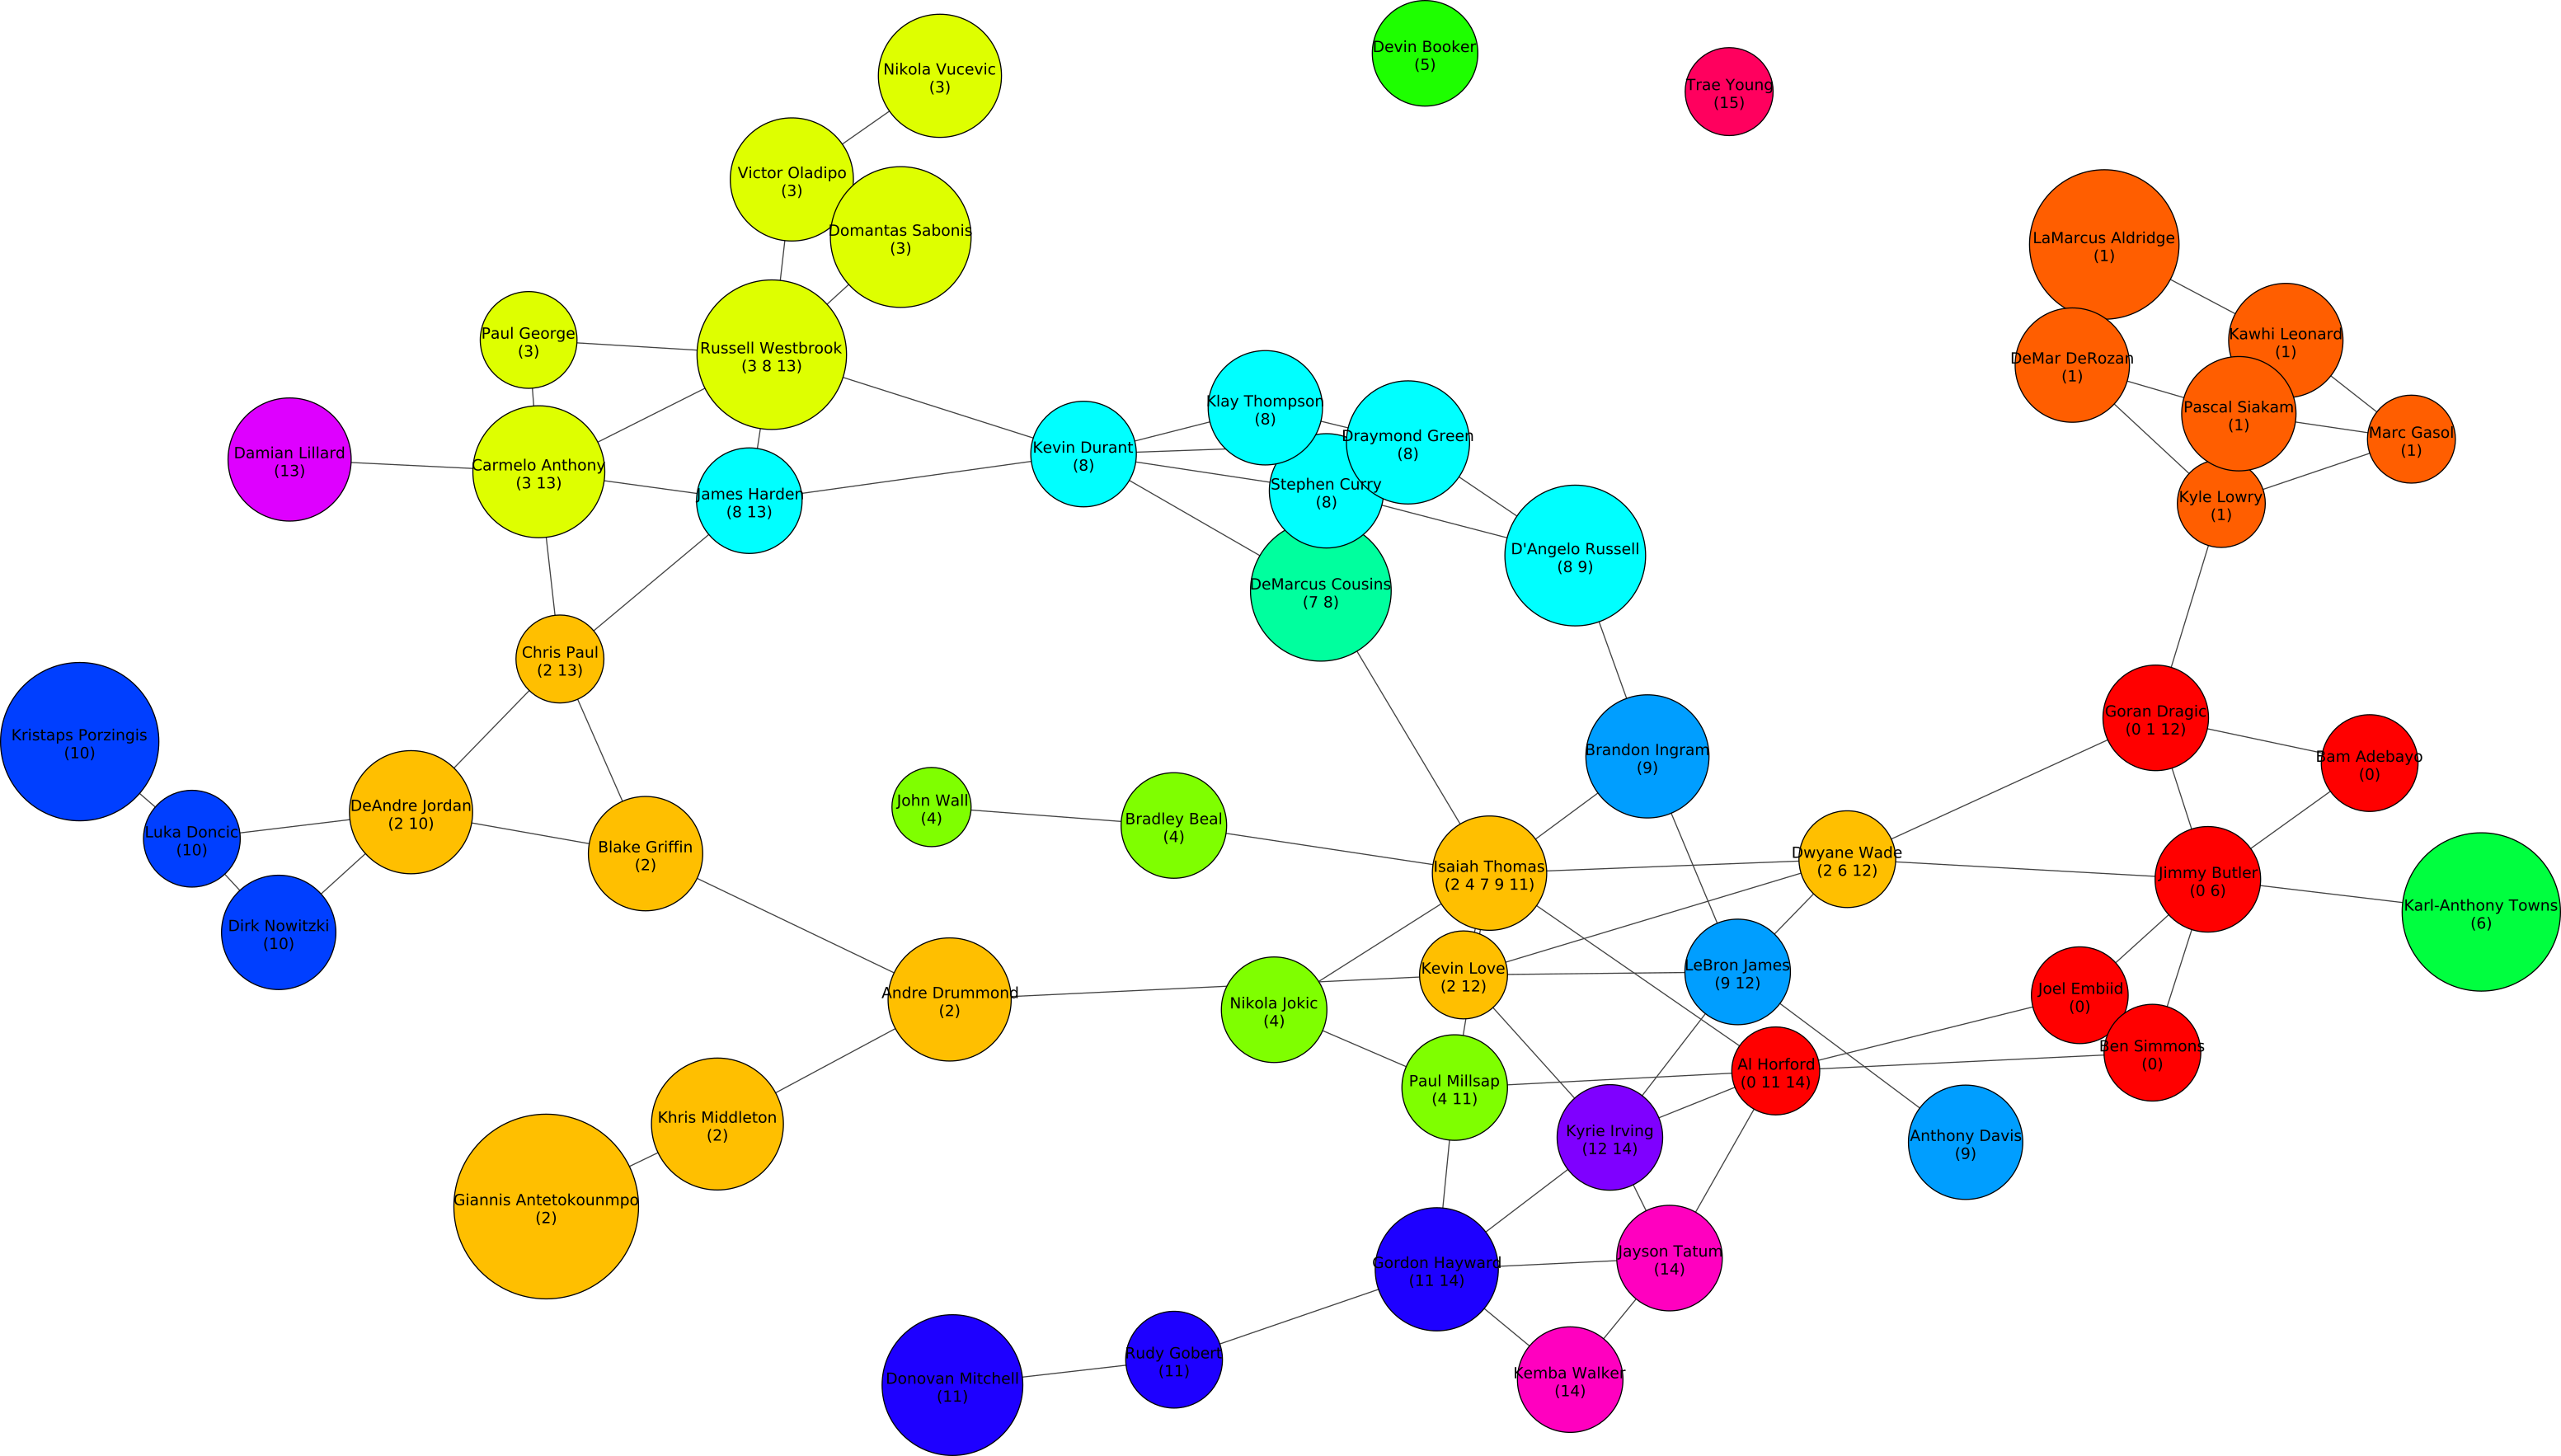
\includegraphics[width=\textwidth]{images/is-sample-2.png}
\caption{Modularność na poziomie 0.3 wśród maksimów}
\end{figure}

\begin{figure}[H]
\centering
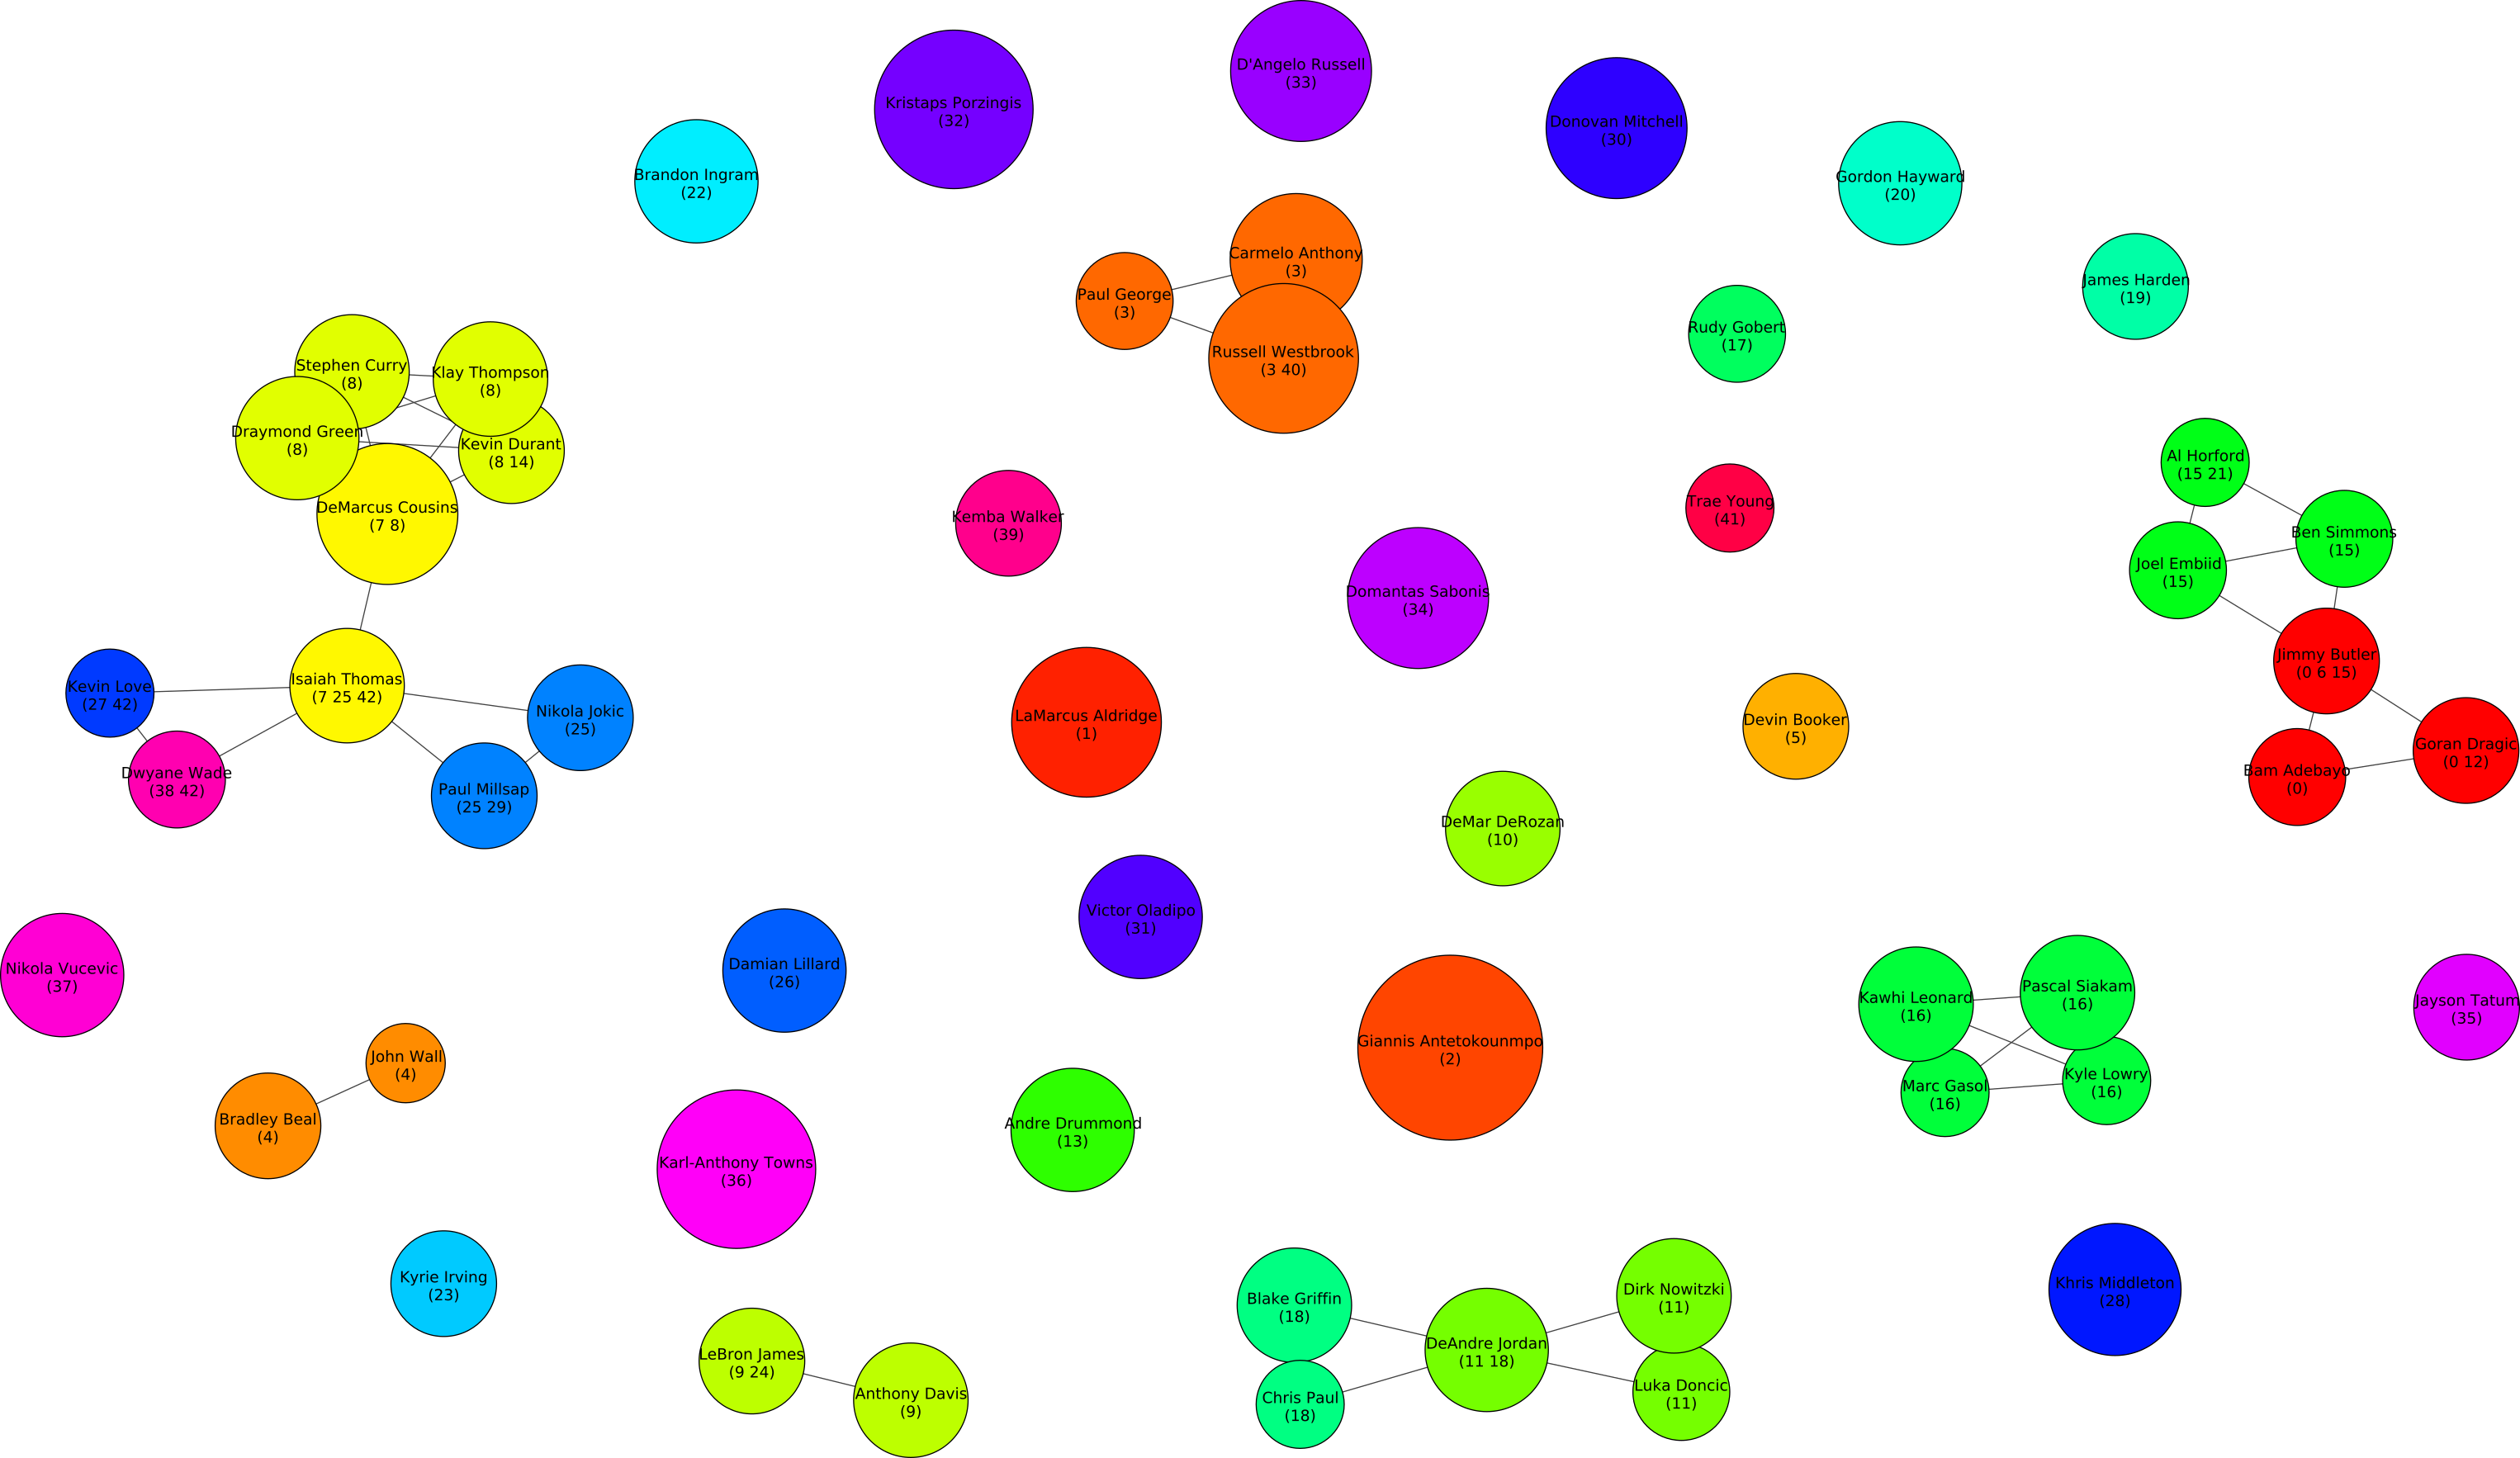
\includegraphics[width=\textwidth]{images/is-sample-3.png}
\caption{Najmniejsza modularność pośród maksimów}
\end{figure}

Powyższe przykłady idealnie obrazują, jak zmienia się rezultat w zależności od maksimum lokalnego, które wybierzemy. Widać jednocześnie, że dla najwyższej wartości modularności uzyskano grupy największe pod względem średniej liczby członków. Gdyby jednak poszukiwane grupy okazały się zbyt duże, manipulacja kwantylem pozwoli zmniejszyć ich rozmiar. I tak dla najmniejszego z maksimów graf wynikowy wskaże nam małe grupy, które jednak są najbardziej ściśle z sobą związane. \\
Jest to moment, w którym możemy wskazać duży atut algorytmu CONGA. Właśnie poprzez manipulację współczynnikiem kwantylu możemy w łatwy sposób manipulować wynikiem, jaki jest według nas najlepszy. Posiadając wynikowy dendrogram operacja uzyskiwania grafu wynikowego jest operacją liniową. Dzięki temu możemy odzyskać graf z każdego z kroków algorytmu w bardzo prosty sposób. Ułatwia to nie tylko implementacje, lecz także odnalezienie skali grup, jakich oczekiwał użytkownik. \\
Warto zaznaczyć, że podczas prezentacji wyników skorzystano z własności maksimum lokalnego. Nic jednak nie stoi na przeszkodzie, aby odzyskać graf wynikowe w bardziej 'prymitywny' sposób. Jednym z nich może być po prostu wybór numeru jednej z iteracji. W dendrogramie podczas każdego kroku rozmiary społeczności wynikowych trzymają się tendencji malejącej. Tak więc im dalszy krok algorytmu wybierzemy, tym graf wynikowy będzie posiadał społeczności mniejszych rozmiarów. \\
Wielkość grup można określić poprzez parametr modularności (tutaj jednak najwyższa wartość nie jest jednak ściśle związana z rozmiarem grupy), natomiast skalę nakładania się społeczności można modyfikować poprzez wykonanie preprocessingu (ta operacja jest jednak bardzo kosztowna, ponieważ de facto dwa razy wykonujemy sam algorytm, jedynie ograniczając liczbę iteracji podczas drugiego wykonania). Sam preprocessingu można również przeprowadzić 'samodzielnie' poprzez określenie pewnej wartości handicapu, jaki usuwanie krawędzi ma nad kopiowaniem wierzchołka. Wariant ten prezentuje poniższy przykład.\\

\begin{figure}[H]
\centering
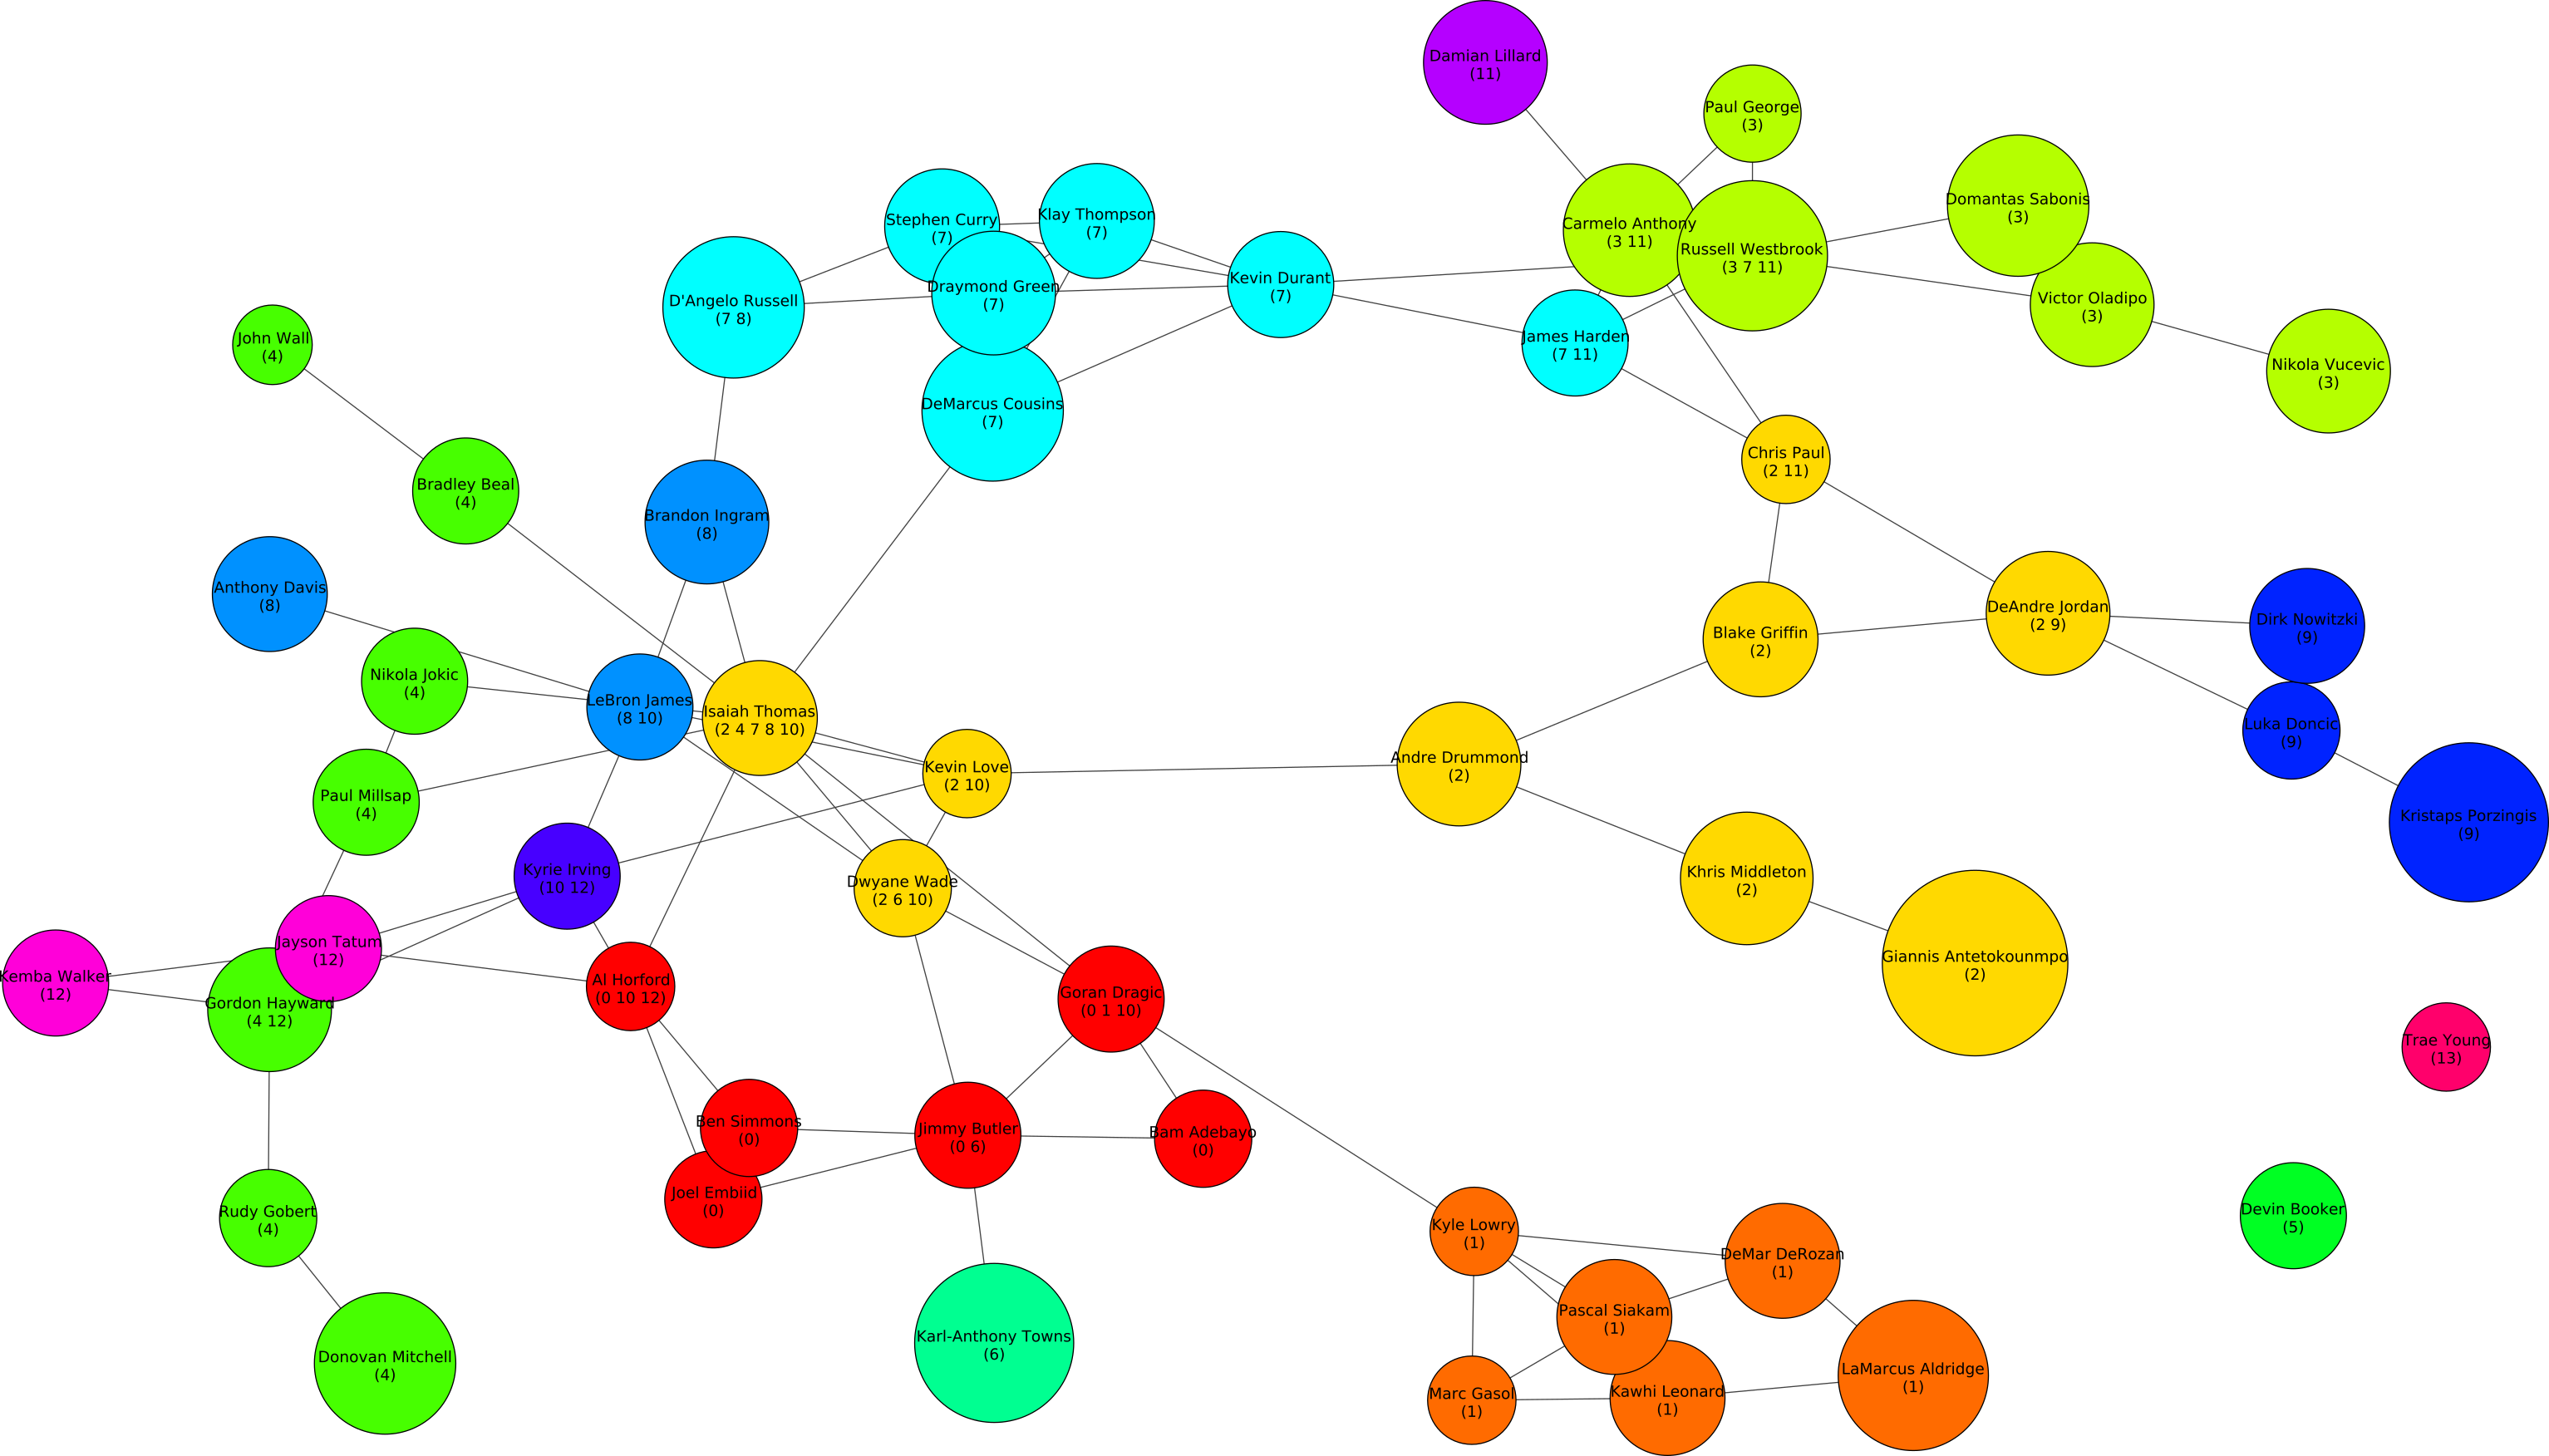
\includegraphics[width=\textwidth]{images/is-sample-4.png}
\caption{Wynik przy gap=5 (największa wartość modularności)}
\end{figure}

Graf przedstawiony powyżej został wygenerowany z tego samego grafu początkowego co grafy z rysunków 1, 2 i 3. Prezentowany wynik to wynik dla iteracji o największej wartości modularności. Można zauważyć, iż rezultat ten jest zbliżony do grafu, który został uzyskany przy kwantylu 0.3 dla poprzedniego sposobu wyznaczania wyniku. Parametr gap ogranicza w naszym przypadku liczbę społeczności nachodzących, jednak zachwiana jest w ten sposób tendencja parametru modularności. Przy braku handicapu modularność dla kolejnych iteracji maleje, tutaj tracimy tę własność. Spójrzmy na wynik uzyskany dla kwantylu 0.3.

\begin{figure}[H]
\centering
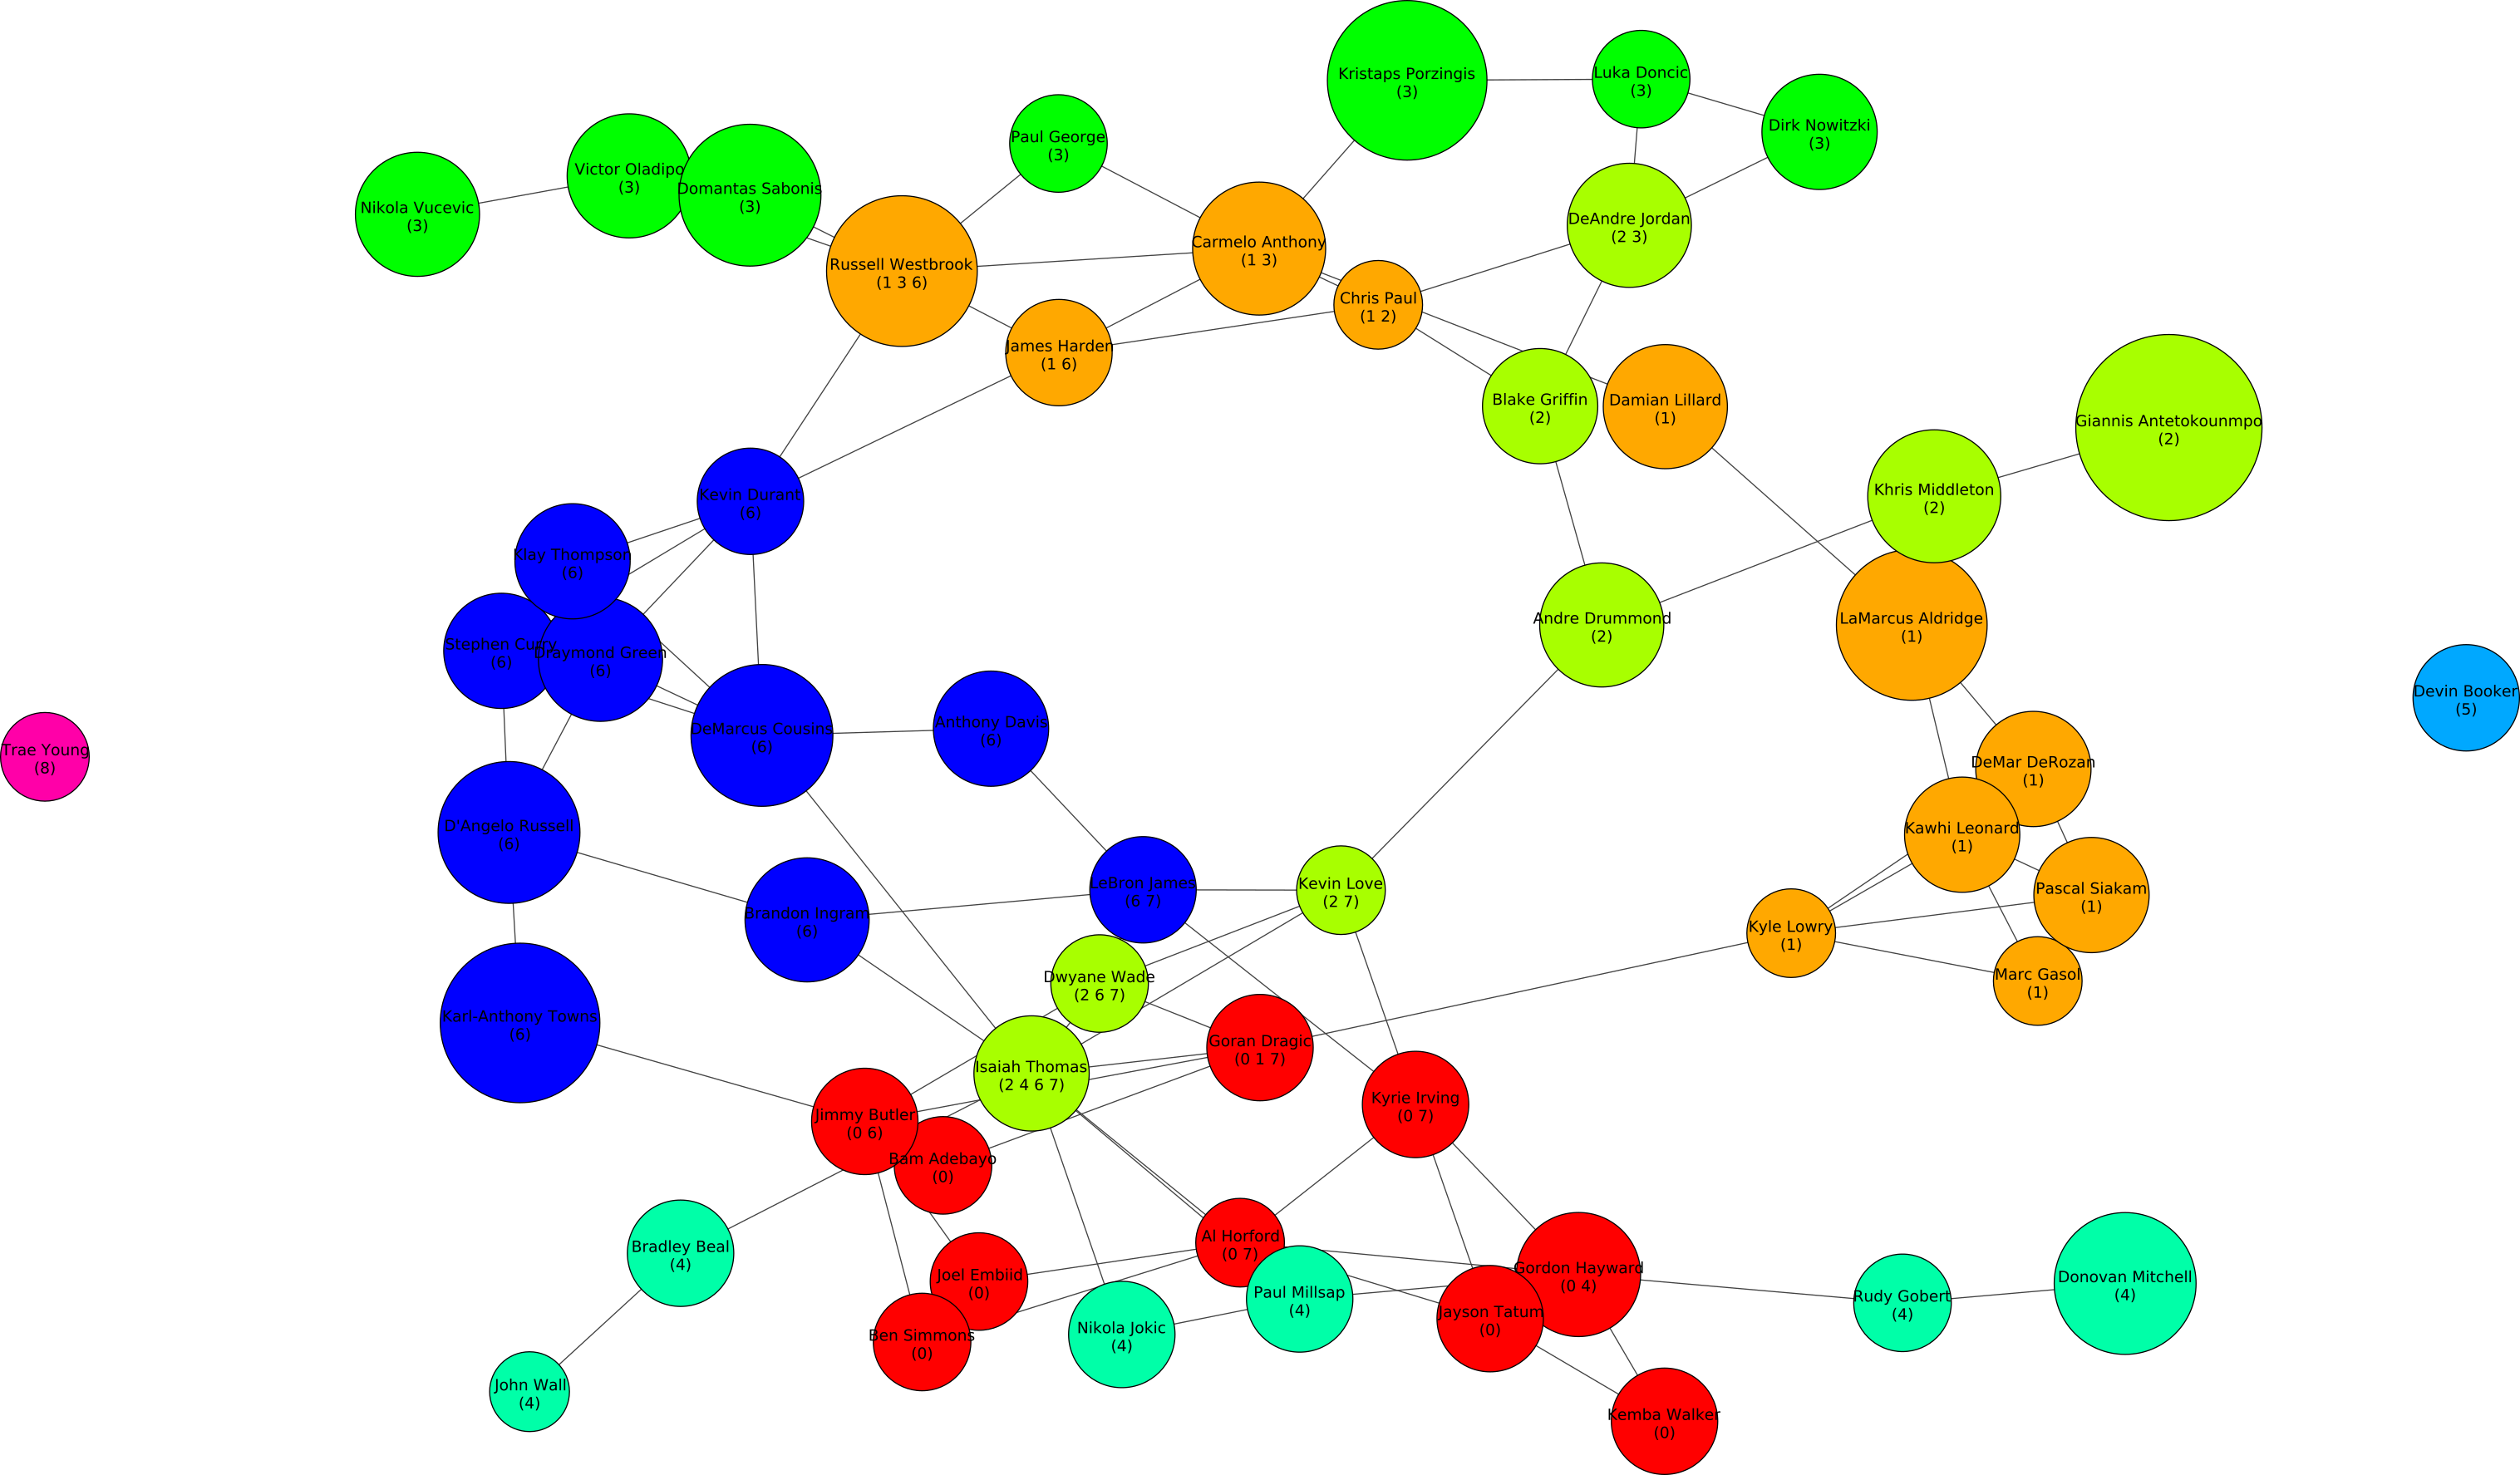
\includegraphics[width=\textwidth]{images/is-sample-5.png}
\caption{Wynik przy gap=5 i kwantylu 0.3}
\end{figure}

Widać więc, że dla prezentowanego maksimum społeczności są większych rozmiarów aniżeli dla wyniku osiągniętego przy największej modularności. W przypadku tak małego grafu ciężko zauważyć różnice na poziomie średniej liczby społeczności dla danego wierzchołka. Przy większych grafach zachowanie to jest jednak zauważalne. \\
To prowadzi do kolejnej obserwacji poczynionej podczas badania algorytmu. Początkową fazę jego działania w głównej mierze stanowi kopiowanie wierzchołka. Jest to oczywiście zależne od wielkości grafu, a także jego gęstości, jednak wszędzie na początku działania algorytmu dokonywania jest seria kopii wierzchołka. Jednocześnie różnica pomiędzy wartościami edge betweenness i vertex betweenness maleje z wykonaniem każdej kolejnej kopii aż do wykonania pierwszego usunięcia krawędzi. Samo usuwanie krawędzi miało odbywać się w jednej iteracji dla wszystkich tych, które mają największy parametr edge betweenness. W rzeczywistości krok te sprowadzał się niemal dla każdej iteracji usunięciem tylko jednej krawędzi, ponieważ przy dużych grafach parametr edge betweenness był bardzo zróżnicowany dla każdej z krawędzi. Dopiero przy ostatnich iteracjach krawędzie usuwane były grupowo (zazwyczaj były to bardzo liczne grupy). \\
Wracając do przykładu, wywołanie algorytmu w ten sposób na pewno przyniesie za sobą korzyść czasową. Jednocześnie jednak należy pamiętać, iż jest to równoznaczne z innym przebiegiem algorytmu. W tym wariancie parametr początkowy wpływa w głównej mierze na liczbe społeczności, do jakiej należy jeden wierzchołek. Im większy handicap na korzyść parametru edge betweenneess tym mniej podziałów na społeczności nachodzące, a co za tym idzie także większe rozmiary społeczności docelowych.\\
W tym miejscu warto także wspomnieć o rezultatach, jakie udało się osiągnąć, dzięki wprowadzonym modyfikacjom. Posiadanie parametrów dat zawarcia znajomości znacznie ułatwiło proces podziału wierzchołka na oryginał i kopię zarówno od strony implementacyjnej, jak i logiki, która za tym stała. Modyfikacja wyłącznie po latach zawarcia znajomości miała na celu wyłonienie grupy tylko na podstawie daty zawarcia znajomości, a więc opierając się na założeniu, że grupę można identyfikować poprzez bliskie sobie daty zawarcia znajomości wśród jej uczestników. Dodając wagę w postaci liczby wspólnych znajomych przeniesiono nacisk na fakt przebywania dłużej w tej samej grupie - jeśli dwie osoby dłużej przebywają w tym samym otoczeniu, tym ich liczba wspólnych znajomych wzrasta.\\
Analiza obu modyfikacji pod względem parametru modularności nie wskazała znacznych różnic zależnych od modyfikacji. W tym wypadku do analizy wykorzystano wiedzę ekspercką na temat grafu zawodników NBA. Posłużmy się więc przykładem:

\begin{figure}[H]
\centering
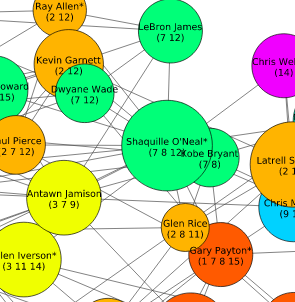
\includegraphics[width=\textwidth]{images/is-sample-6.png}
\caption{Modyfikacja z rokiem zawarcia znajomości}
\end{figure}

\begin{figure}[H]
\centering
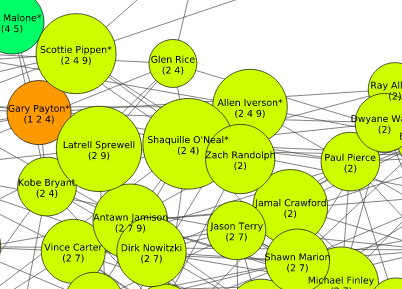
\includegraphics[width=\textwidth]{images/is-sample-7.png}
\caption{Modyfikacja z rokiem zawarcia znajomości i ze wspólną liczbą znajomych}
\end{figure}

Prezentowany przykład skupia się na osobie koszykarza Shaquille O'Neala. Zawodnik ten jest niezwykle utytułowany, a w swej karierze zwiedził mnóstwo klubów. Na wstępie warto zaznaczyć, iż wynik brany tutaj pod uwagę został wybrany na podstawie największe wartości modularności. Na tym przykładzie możemy zaobserwować, iż przy uwzględnieniu liczby wspólnych znajomych społeczność wynikowa stała się bardzo liczna. Wynika to z faktu, iż podczas swej kariery analizowany zawodnik zdążył zagrać w jednym klubie z wieloma innymi koszykarzami, przez co z wieloma z nich miał dużą liczbę wspólnych znajomych. Gdy ten parametr pominiemy podany zawodnik znajdzie się w 3 społecznościach. Ponadto jedna z nich wyraźnie wskazuje na zespół Los Angeles Lakers, do którego O'Neal dołączył w roku 1996. \\
Podobnych przykładów można znaleźć znacznie więcej w zależności od grafu, który analizujemy. Wskazują one, że dodanie liczby wspólnych znajomych jako wagi rzeczywiście wpływa na rozkład grup. Dysponując wiedzą na temat wierzchołków i realnych zależności można skupić się na analizie pojedynczych wierzchołków, jednak obserwacje w skali makro również przynoszą pewne wnioski. Podchodząc do problemu w ten sposób można zauważyć, iż w przypadku dodania wag krawędzi wynik 'spłaszcza się', zwracając mniej społeczności, które są za to bardziej liczne. Skorzystanie z samej daty zawarcia znajomości dzieli graf na mniejsze społeczności. \\
Warto w tym miejscu wspomnieć jednak o tym, iż uzyskany wynik niekoniecznie jest zobowiązujący. W przypadku uzyskania zbyt dużych społeczności modyfikacja wyboru maksimum lokalnego zgodnie z obserwacjami poczynionymi w poprzednich akapitach. Algorytm CONGA daje bardzo dużą elastyczność w kwestii uzyskanych wyników. Modyfikacje, które zostały wykonane w głównej mierze skupiają się na rezultacie końcowyw. Ten jednak oparty jest na mierze modularności, która nie jest jednak w żaden sposób miarą wiążącą. W przypadku tego algorytmu to użytkownik 'decyduje', jaki podział na grupy według niego będzie najlepszy. Jeżeli oczywiście tylko cierpliwość pozwoli mu na odczekanie końca działania algorytmu.

\begin{figure}[H]
\centering
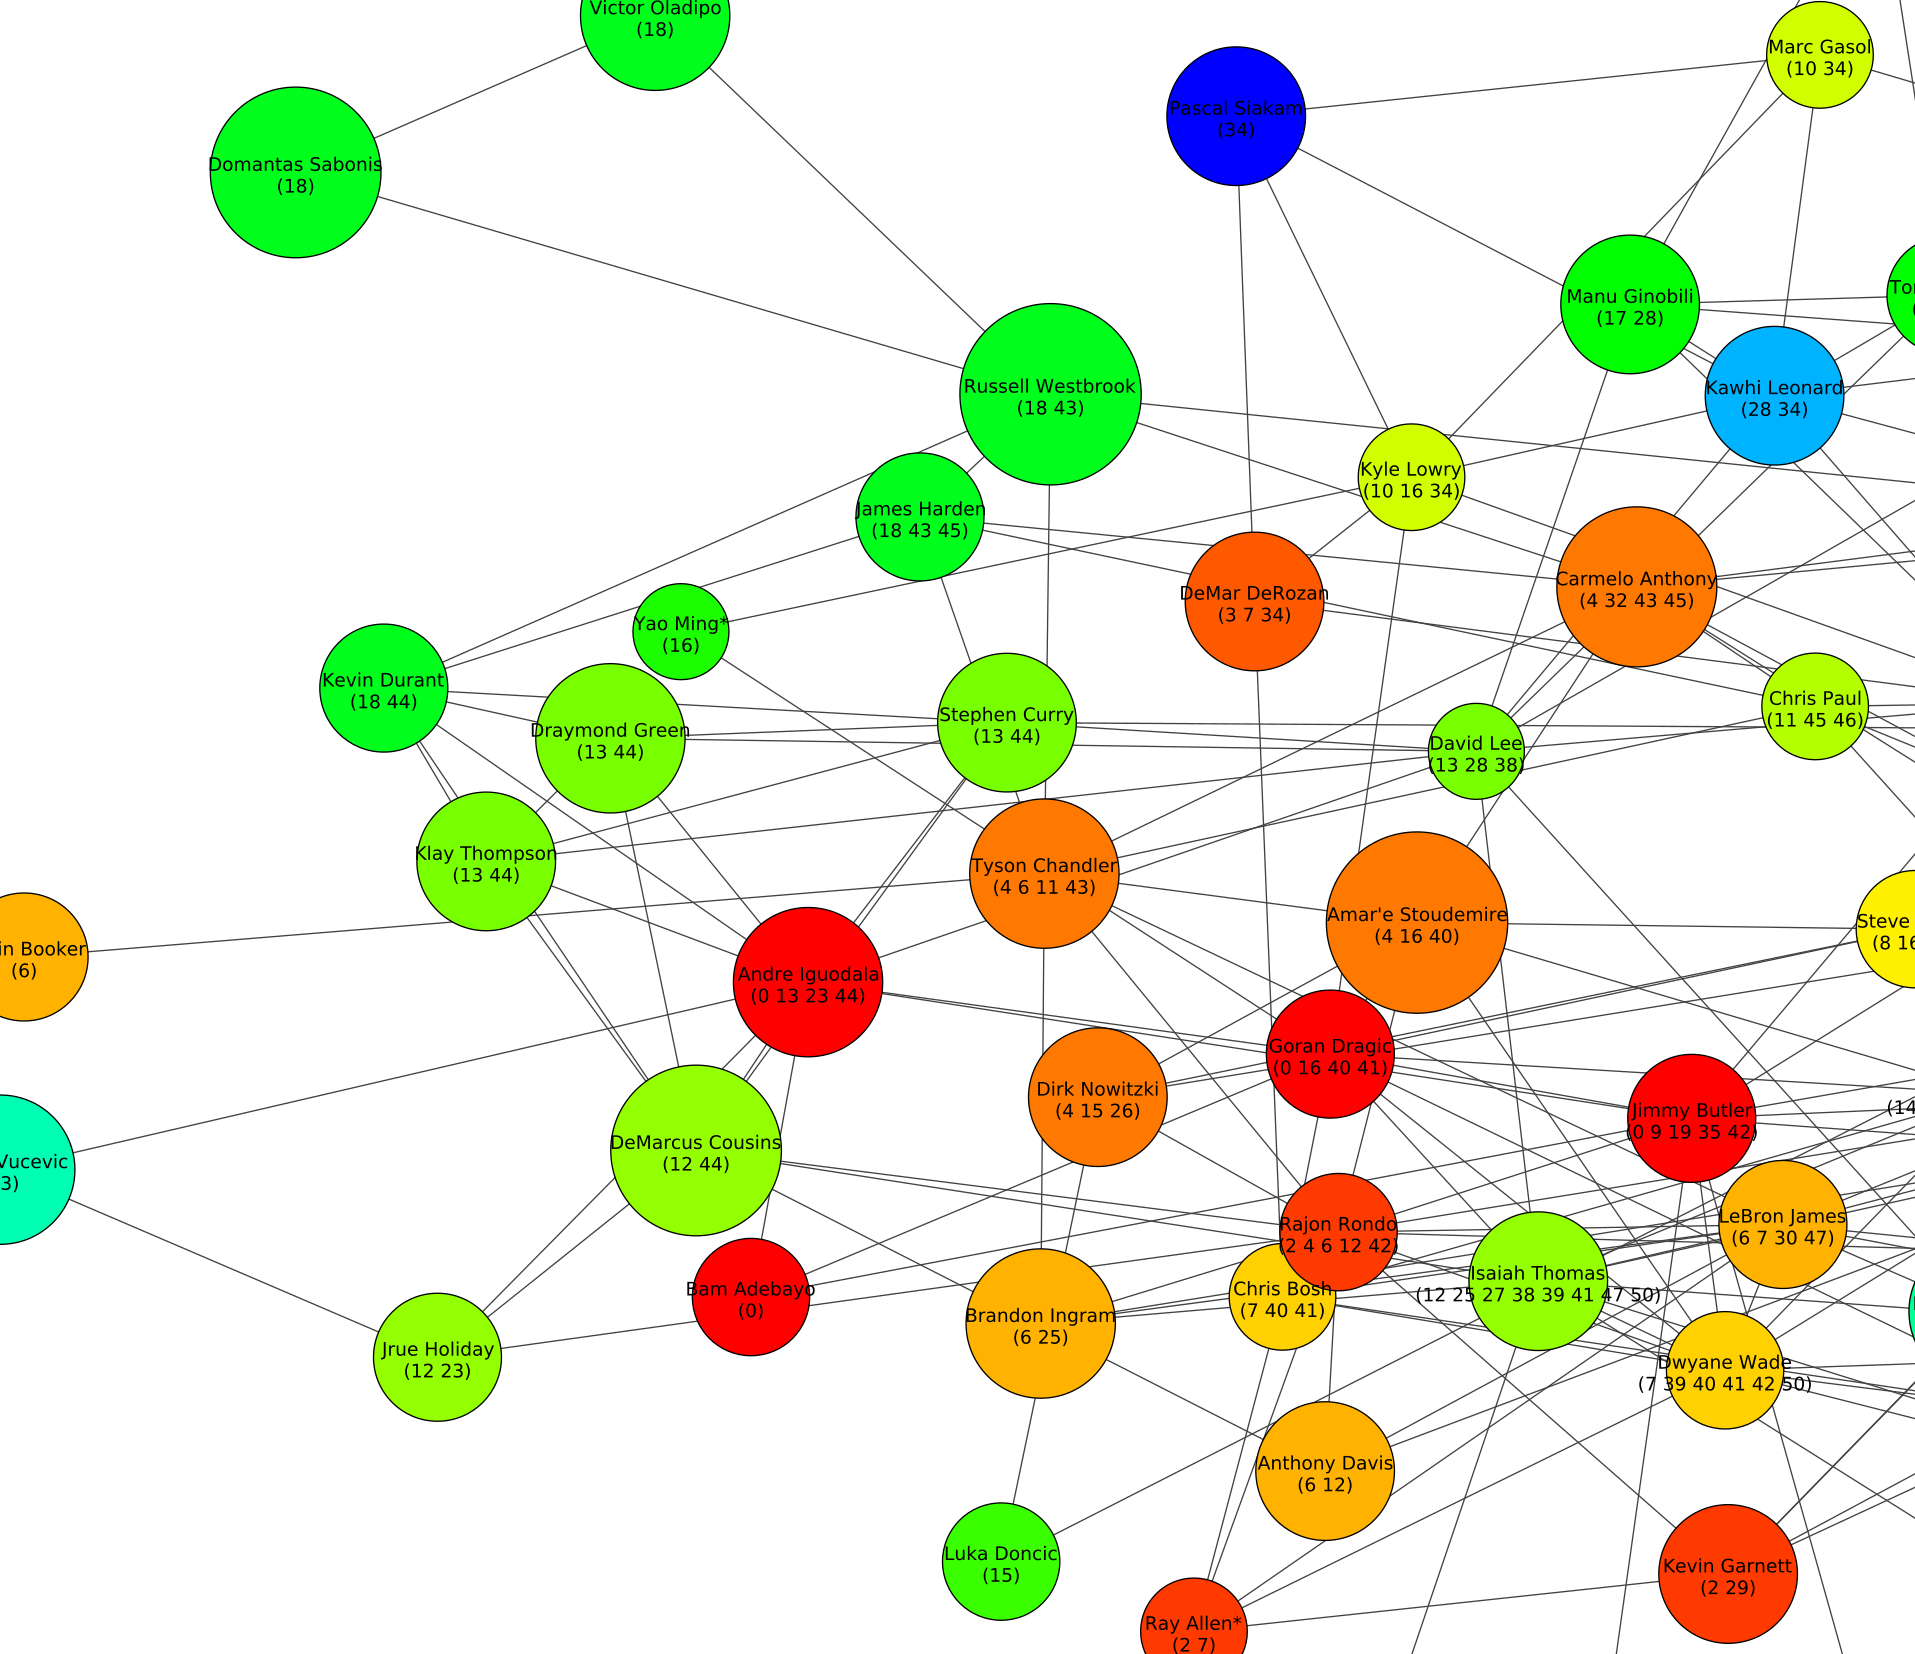
\includegraphics[width=\textwidth]{images/ms-image-sample.png}
\caption{Przykładowe wyjście}
\end{figure}

%-----------------------------------------------------%
%LPA
%-----------------------------------------------------%
\subsection{Label Propagation Algorithm}
\subsubsection{Analiza czasowa}
Algorytm LPA, zgodnie z oczekiwaniami, okazał się być algorytmem wystarczająco szybkim, aby przeprowadzić obliczenia na wszystkich zbiorach danych w projekcie.

\subsubsection{Analiza jakościowa}


%-----------------------------------------------------%
%OCDLCE
%-----------------------------------------------------%
\subsection{Overlapping Community Detection by Local Community Expansion}
\subsubsection{Analiza czasowa}
\subsubsection{Analiza jakościowa}

%-----------------------------------------------------%
%Louvain
%-----------------------------------------------------%
\subsection{Algorytm Louvain}
\subsubsection{Analiza czasowa}
\subsubsection{Analiza jakościowa}

%-----------------------------------------------------%
%Porównanie
%-----------------------------------------------------%
\subsection{Porównanie}

%-----------------------------------------------------%
%Wnioski
%-----------------------------------------------------%
\subsection{Wnioski}

\newpage
\printbibliography

\end{document}

